\documentclass[11pt,a4paper]{article}
\usepackage[utf8]{inputenc}
\usepackage[T1]{fontenc}
\usepackage[sc]{mathpazo}
\usepackage[scaled=0.92]{helvet}
\usepackage{microtype}
\usepackage[a4paper,top=2.6cm,bottom=2.4cm,left=2.4cm,right=2.4cm,headheight=14pt]{geometry}
\usepackage[table]{xcolor}
\usepackage{booktabs,array,enumitem,multirow}
\usepackage{tikz}
\usetikzlibrary{calc,positioning}
\usepackage{pgfplots}
\pgfplotsset{compat=1.16}
\usepackage[most]{tcolorbox}
\usepackage{titlesec}
\usepackage{needspace,etoolbox}
\usepackage{fancyhdr}
\usepackage{caption}
\usepackage{url}
\def\UrlBreaks{\do\/\do\-\do\_\do\.\do\=\do\?\do\&\do\a\do\b\do\c\do\d\do\e\do\f\do\g\do\h\do\i\do\j\do\k\do\l\do\m\do\n\do\o\do\p\do\q\do\r\do\s\do\t\do\u\do\v\do\w\do\x\do\y\do\z}
\Urlmuskip=0mu plus 1mu
\urlstyle{same}
\usepackage[hidelinks]{hyperref}

% ---- Palet (selaras dengan halaman dokumen pelengkap) ----
\definecolor{teal}{HTML}{0A6C6E}
\definecolor{tealdark}{HTML}{07484A}
\definecolor{ink}{HTML}{13262A}
\definecolor{muted}{HTML}{51666A}
\definecolor{rule}{HTML}{D3DEDC}
\definecolor{pale}{HTML}{EEF5F4}
\definecolor{amber}{HTML}{B7791F}
\definecolor{amberpale}{HTML}{FBF4E4}
\definecolor{well}{HTML}{CFE3E0}

\renewcommand{\tablename}{Tabel}
\renewcommand{\figurename}{Gambar}
\renewcommand{\refname}{Daftar Pustaka}
\color{ink}
\setlength{\parindent}{0pt}
\setlength{\parskip}{6.5pt plus 1pt}
\linespread{1.06}
\tolerance=1200
\emergencystretch=3em
\hyphenpenalty=1500
\setlist{itemsep=2.5pt,topsep=3pt,parsep=0pt,leftmargin=1.4em}
\setlist[itemize]{label={\color{teal}\textbullet}}
\renewcommand{\arraystretch}{1.22}
\setlength{\tabcolsep}{5pt}
\captionsetup{font={small,sf,color=muted},labelfont={bf,color=teal},labelsep=period,justification=raggedright,singlelinecheck=false,skip=5pt}

% ---- Judul bagian ----
\titleformat{\section}{\sffamily\bfseries\Large\color{ink}}{\color{teal}\thesection}{0.7em}{}[{\color{rule}\titlerule[0.6pt]}]
\titlespacing*{\section}{0pt}{18pt}{9pt}
\titleformat{\subsection}{\sffamily\bfseries\normalsize\color{tealdark}}{\color{teal}\thesubsection}{0.6em}{}
\titlespacing*{\subsection}{0pt}{11pt}{3pt}

% ---- Kepala dan kaki halaman ----
\pagestyle{fancy}
\fancyhf{}
\renewcommand{\headrulewidth}{0pt}
\fancyhead[L]{\sffamily\scriptsize\color{muted}\textsc{Alergen}\ \raisebox{0.15ex}{\tiny$\bullet$}\ Spesifikasi Produk}
\fancyhead[R]{\sffamily\scriptsize\color{muted}Kit Diagnostik Alergi Berbasis Patch}
\fancyfoot[L]{\sffamily\scriptsize\color{muted}Universitas Airlangga \ $\cdot$ \ IDS000011522}
\fancyfoot[R]{\sffamily\small\bfseries\color{teal}\thepage}
\renewcommand{\headrule}{\color{rule}\hrule width\headwidth height 0.5pt}
\renewcommand{\headrulewidth}{0.5pt}
\fancypagestyle{plain}{\fancyhf{}\renewcommand{\headrulewidth}{0pt}\fancyfoot[R]{\sffamily\small\bfseries\color{teal}\thepage}}

% ---- Tabel ----
\newcommand{\tH}[1]{\textcolor{white}{\sffamily\bfseries\small #1}}
\newcommand{\tabstart}{\small\rowcolors{2}{white}{pale}\arrayrulecolor{rule}}
\newcommand{\hdrrow}{\rowcolor{tealdark}}
\newcolumntype{L}[1]{>{\raggedright\arraybackslash}p{#1}}
\newcolumntype{R}[1]{>{\raggedleft\arraybackslash}p{#1}}
\setlength{\aboverulesep}{0pt}\setlength{\belowrulesep}{0pt}
\renewcommand{\toprule}{\arrayrulecolor{tealdark}\specialrule{0.9pt}{0pt}{0pt}\arrayrulecolor{rule}}
\renewcommand{\bottomrule}{\arrayrulecolor{tealdark}\specialrule{0.9pt}{0pt}{0pt}\arrayrulecolor{rule}}

% ---- Kotak catatan dan kartu angka ----
\newtcolorbox{catatan}[1][Catatan]{enhanced,breakable,colback=amberpale,colframe=amberpale,boxrule=0pt,
  borderline west={2.2pt}{0pt}{amber},arc=1.5pt,left=10pt,right=8pt,top=6pt,bottom=6pt,
  before skip=8pt,after skip=10pt,
  title={\sffamily\bfseries\small\color{amber}\MakeUppercase{#1}},coltitle=amber,
  attach boxed title to top left={yshift=-2mm,xshift=0pt},boxed title style={empty,left=0pt,top=0pt,bottom=0pt},
  fonttitle=\sffamily,coltext=ink,before upper={\vspace{2pt}}}
\newtcolorbox{kartu}[2]{enhanced,colback=pale,colframe=pale,boxrule=0pt,arc=3pt,
  left=8pt,right=6pt,top=6pt,bottom=6pt,halign=left,
  borderline west={2.5pt}{0pt}{teal},
  before upper={{\sffamily\bfseries\LARGE\color{teal}#1}\par\vspace{1pt}},
  fontupper=\sffamily\scriptsize\color{muted},height=1.95cm,valign=top}
\newcommand{\kartuRow}[4]{%
 \begin{tcbraster}[raster columns=#1,raster equal height,raster column skip=7pt,raster row skip=7pt]#2#3#4\end{tcbraster}\vspace{9pt}}

% ---- Sampul ----
\newcommand{\patchmotif}[2]{% #1 skala, #2 warna garis
 \begin{scope}[scale=#1]
 \draw[#2,line width=1.2pt,rounded corners=9pt] (0,0) rectangle (15,6);
 \foreach \r in {0,1}{\foreach \c in {0,...,4}{
   \draw[#2,line width=1pt] ({1.9+\c*2.7},{4.1-\r*2.2}) circle (0.9);}}
 \end{scope}}

\newcommand{\makecover}[5]{% kode, judul, subjudul, tagline, ringkasan satu kalimat
\begin{titlepage}
\thispagestyle{empty}
\begin{tikzpicture}[remember picture,overlay]
 \fill[tealdark] (current page.north west) rectangle ($(current page.north east)+(0,-17.2cm)$);
 \fill[teal!85!tealdark] ($(current page.north east)+(0,-17.2cm)$) -- ($(current page.north east)+(-10cm,-17.2cm)$) -- ($(current page.north east)+(0,-10.8cm)$) -- cycle;
 \begin{scope}[shift={($(current page.north east)+(-9.9cm,-6.4cm)$)}]
   \patchmotif{0.5}{white!35}
 \end{scope}
 \node[anchor=north west,text=white!70,font=\sffamily\small\bfseries,align=left] at ($(current page.north west)+(2.4cm,-2.7cm)$) {\textsc{Alergen \ $\cdot$ \ Universitas Airlangga}};
 \node[anchor=north west,text=white,font=\sffamily\bfseries\fontsize{44}{44}\selectfont] at ($(current page.north west)+(2.4cm,-7.4cm)$) {#1};
 \node[anchor=north west,text=white,font=\sffamily\bfseries\fontsize{26}{31}\selectfont,text width=14.2cm,align=left] at ($(current page.north west)+(2.4cm,-10.2cm)$) {#2};
 \node[anchor=north west,text=white!85,font=\sffamily\fontsize{13}{17}\selectfont,text width=14cm,align=left] at ($(current page.north west)+(2.4cm,-14.1cm)$) {\hyphenpenalty=10000\exhyphenpenalty=10000 #3};
 \node[anchor=north west,text=ink,font=\fontsize{12}{17}\selectfont,text width=15.2cm,align=left] at ($(current page.north west)+(2.4cm,-18.8cm)$) {#4};
 \draw[teal,line width=2pt] ($(current page.north west)+(2.4cm,-21.9cm)$) -- ++(2.2cm,0);
 \node[anchor=north west,text=muted,font=\sffamily\small,text width=15cm,align=left] at ($(current page.north west)+(2.4cm,-22.4cm)$) {%
  \textbf{\color{ink}Kit Diagnostik Alergi Berbasis Patch (Alergen)}\\[3pt]
  Universitas Airlangga, Surabaya\\
  Paten Sederhana IDS000011522\\
  Oktober 2026};
 \node[anchor=south east,text=muted,font=\sffamily\scriptsize,align=right] at ($(current page.south east)+(-2.4cm,1.6cm)$) {#5};
\end{tikzpicture}
\end{titlepage}
\newpage}

\definecolor{sr1}{HTML}{8AA6AB}
\definecolor{sr2}{HTML}{3FA7A3}
\definecolor{sr3}{HTML}{0A6C6E}
\definecolor{sr4}{HTML}{B7791F}
\pgfplotsset{natbase/.style={width=0.95\linewidth,height=6.2cm,
  every axis label/.append style={font=\sffamily\scriptsize,color=muted},
  tick label style={font=\sffamily\scriptsize,color=muted},
  legend style={font=\sffamily\scriptsize,draw=rule,fill=white,at={(0.5,-0.2)},anchor=north},
  grid=major,grid style={color=rule,line width=0.4pt},
  axis line style={color=rule},tick style={color=rule},
  scaled ticks=false,/pgf/number format/.cd,1000 sep={.},fixed,precision=0,/tikz/.cd},
  natplot/.style={natbase,xtick={1,2,3,4,5},xticklabels={2028,2029,2030,2031,2032}}}
\hypersetup{pdftitle={Spesifikasi Produk},pdfauthor={Tim Alergen, Universitas Airlangga}}

\pretocmd{\section}{\Needspace{7\baselineskip}}{}{}
\pretocmd{\subsection}{\Needspace{4\baselineskip}}{}{}

\usepackage{float}
\begin{document}

\makecover{Produk}{Spesifikasi Produk}{Patch Alergen: kit diagnostik alergi berbasis patch dengan sepuluh alergen}{Dokumen ini menetapkan spesifikasi produk patch Alergen: identitas dan penggunaan yang dituju, konfigurasi fisik, bahan, kandungan alergen per sumur, kriteria mutu, kemasan, penandaan, penyimpanan, dan batasan pemakaian.}{Patch 2 $\times$ 5 cm, 10 sumur, 30 $\mu$g protein per alergen}

\section*{Ringkasan}
\addcontentsline{toc}{section}{Ringkasan}

\kartuRow{4}
{\begin{kartu}{10}{}alergen, masing-masing pada sumur sendiri\end{kartu}}
{\begin{kartu}{2 $\times$ 5 cm}{}ukuran patch, sumur berdiameter 7 mm\end{kartu}}
{\begin{kartu}{30 $\mu$g}{}protein per alergen per sumur, batas 24 sampai 36 $\mu$g\end{kartu}
\begin{kartu}{12 bln}{}masa simpan pada 2 sampai 8 $^\circ$C\end{kartu}}

Alergen adalah kit diagnostik alergi berbasis patch untuk penapisan reaksi kulit terhadap sepuluh alergen yang umum: tungau debu rumah, udang, susu sapi, daging sapi, daging ayam, putih telur, gandum, kacang tanah, kelapa, dan polen rumput bermuda. Reaksi kulit pada tiap sumur dibaca dari foto patch dengan aplikasi seluler. Produk dilindungi Paten Sederhana IDS000011522.

\section{Identitas dan penggunaan yang dituju}

\begin{table}[H]
\centering
\caption{Identitas produk.}
\label{tab:id}
\tabstart
\begin{tabular}{@{}L{4.0cm}L{11.0cm}@{}}
\toprule
\hdrrow\tH{Butir} & \tH{Keterangan} \\
\midrule
Nama produk & Alergen \\
Jenis & Kit diagnostik alergi berbasis patch untuk pemakaian pada kulit \\
Perlindungan & Paten Sederhana IDS000011522 \\
Pemilik dan pengembang & Universitas Airlangga, Surabaya \\
Konfigurasi & Satu patch 2 $\times$ 5 cm dengan 10 sumur, dalam satu kantong foil dan satu kotak \\
Pembacaan hasil & Foto patch dibaca oleh aplikasi seluler yang memberi skor reaksi per sumur \\
Kontak & info@alergen.unair.ac.id \\
\bottomrule
\end{tabular}
\end{table}

\subsection{Penggunaan yang dituju}

Patch dipakai untuk menapis sensitisasi terhadap sepuluh alergen pada pasien yang dicurigai alergi, dengan hasil dibaca pada tiap sumur dan diinterpretasikan oleh tenaga kesehatan. Hasil patch adalah penapisan, bukan diagnosis tunggal: keputusan klinis tetap memadukan riwayat, pemeriksaan fisik, dan tes lain. Cakupannya sepuluh alergen, sehingga alergi di luar sepuluh alergen itu memerlukan pemeriksaan lain.

Lama tempel, waktu pembacaan, lokasi pemasangan, populasi pengguna, dan kinerja diagnostik (sensitivitas dan spesifisitas) ditetapkan melalui studi validasi klinis. Produk masih berupa prototipe tanpa validasi pada manusia dan belum memiliki izin edar.

\section{Konfigurasi fisik}

Gambar~\ref{fig:patch} memperlihatkan tata letak sepuluh sumur dalam dua baris, nomor 1 sampai 5 di baris atas dan 6 sampai 10 di baris bawah. Urutan alergen per sumur ada pada Tabel~\ref{tab:sumur}.

\begin{figure}[H]
\centering
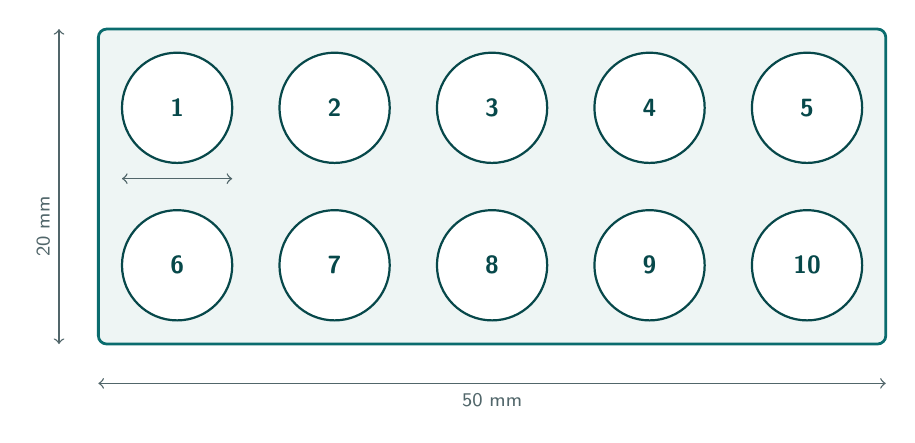
\begin{tikzpicture}[x=2cm,y=2cm]
\draw[teal,line width=1pt,rounded corners=3pt,fill=pale] (0,0) rectangle (5,2);
\draw[tealdark,line width=0.8pt,fill=white] (0.5,1.5) circle (0.35);
\node[font=\sffamily\bfseries\small,text=tealdark] at (0.5,1.5) {1};
\draw[tealdark,line width=0.8pt,fill=white] (1.5,1.5) circle (0.35);
\node[font=\sffamily\bfseries\small,text=tealdark] at (1.5,1.5) {2};
\draw[tealdark,line width=0.8pt,fill=white] (2.5,1.5) circle (0.35);
\node[font=\sffamily\bfseries\small,text=tealdark] at (2.5,1.5) {3};
\draw[tealdark,line width=0.8pt,fill=white] (3.5,1.5) circle (0.35);
\node[font=\sffamily\bfseries\small,text=tealdark] at (3.5,1.5) {4};
\draw[tealdark,line width=0.8pt,fill=white] (4.5,1.5) circle (0.35);
\node[font=\sffamily\bfseries\small,text=tealdark] at (4.5,1.5) {5};
\draw[tealdark,line width=0.8pt,fill=white] (0.5,0.5) circle (0.35);
\node[font=\sffamily\bfseries\small,text=tealdark] at (0.5,0.5) {6};
\draw[tealdark,line width=0.8pt,fill=white] (1.5,0.5) circle (0.35);
\node[font=\sffamily\bfseries\small,text=tealdark] at (1.5,0.5) {7};
\draw[tealdark,line width=0.8pt,fill=white] (2.5,0.5) circle (0.35);
\node[font=\sffamily\bfseries\small,text=tealdark] at (2.5,0.5) {8};
\draw[tealdark,line width=0.8pt,fill=white] (3.5,0.5) circle (0.35);
\node[font=\sffamily\bfseries\small,text=tealdark] at (3.5,0.5) {9};
\draw[tealdark,line width=0.8pt,fill=white] (4.5,0.5) circle (0.35);
\node[font=\sffamily\bfseries\small,text=tealdark] at (4.5,0.5) {10};
\draw[<->,muted,line width=0.5pt] (0,-0.25)--(5,-0.25) node[midway,below,font=\sffamily\scriptsize,text=muted]{50 mm};
\draw[<->,muted,line width=0.5pt] (-0.25,0)--(-0.25,2) node[midway,left,font=\sffamily\scriptsize,text=muted,rotate=90,yshift=2mm]{20 mm};
\draw[<->,muted,line width=0.5pt] (0.15,1.05)--(0.85,1.05) node[midway,above,font=\sffamily\tiny,text=muted,yshift=-1pt]{};
\end{tikzpicture}
\caption{Tata letak patch, skala 2:1. Sumur bernomor 1 sampai 10.}
\label{fig:patch}
\end{figure}

\begin{table}[H]
\centering
\caption{Dimensi patch.}
\label{tab:dim}
\tabstart
\begin{tabular}{@{}L{5.0cm}L{4.6cm}L{4.6cm}@{}}
\toprule
\hdrrow\tH{Parameter} & \tH{Nominal} & \tH{Toleransi} \\
\midrule
Panjang & 50 mm & $\pm$ 1 mm \\
Lebar & 20 mm & $\pm$ 1 mm \\
Diameter sumur & 7 mm & $\pm$ 0,3 mm \\
Jumlah sumur & 10 & tetap \\
Susunan sumur & 2 baris $\times$ 5 kolom & sesuai gambar desain \\
\bottomrule
\end{tabular}
\end{table}

\section{Bahan dan konstruksi}

\begin{table}[H]
\centering
\caption{Komponen patch dan kemasan.}
\label{tab:bahan}
{\footnotesize\tabstart\setlength{\tabcolsep}{3.5pt}
\begin{tabular}{@{}L{3.4cm}L{4.6cm}L{6.4cm}@{}}
\toprule
\hdrrow\tH{Komponen} & \tH{Bahan} & \tH{Spesifikasi} \\
\midrule
Lembar penyangga & Film poliester kelas medis & 20 $\times$ 50 mm, permukaan bersih, tidak bereaksi dengan ekstrak \\
Matriks pembawa & Disk penyerap selulosa & Diameter 7 mm, 10 disk, posisi sesuai gambar desain \\
Ekstrak alergen & 10 ekstrak dalam dapar fosfat salin pH 7,4 & Lihat Tabel~\ref{tab:sumur} dan Tabel~\ref{tab:ext} \\
Seal pelindung & Film poliolefin dapat dikelupas & Menutup tiap sumur, daya kupas 1,0 sampai 2,5 N/cm \\
Kantong foil & Laminasi foil aluminium & Penghalang uap air dan cahaya, satu patch per kantong \\
Pengering & Silika gel & Sachet 1 g, bebas debu \\
Kotak & Karton & 3,2 $\times$ 3 cm alas, tinggi 8 cm \\
\bottomrule
\end{tabular}}
\end{table}

\section{Kandungan alergen}

Tiap sumur memuat satu ekstrak alergen sebanyak 30 $\mu$g protein. Tidak ada ekstrak yang dicampur, sehingga tiap alergen diuji dan dikendalikan sendiri \cite{ema}.

\begin{table}[H]
\centering
\caption{Isi tiap sumur.}
\label{tab:sumur}
{\footnotesize\tabstart\setlength{\tabcolsep}{3.5pt}
\begin{tabular}{@{}rL{3.2cm}L{5.0cm}L{4.6cm}@{}}
\toprule
\hdrrow\tH{Sumur} & \tH{Alergen} & \tH{Sumber} & \tH{Penanda utama} \\
\midrule
1 & Tungau debu rumah & \emph{Dermatophagoides pteronyssinus} & Der p 1 \\
2 & Udang & \emph{Penaeus vannamei} & Tropomiosin \\
3 & Susu sapi & Susu sapi segar & Bos d 5 \\
4 & Daging sapi & Otot rangka sapi & Bos d 6 (albumin serum sapi) \\
5 & Daging ayam & Otot dada ayam & Gal d 5 (albumin serum ayam) \\
6 & Putih telur & Putih telur ayam & Ovalbumin (Gal d 2) \\
7 & Gandum & Biji gandum & Gliadin (Tri a 19) \\
8 & Kacang tanah & Biji kacang tanah & Ara h 2 \\
9 & Kelapa & Daging buah kelapa tua & Coc n 1 \\
10 & Polen rumput bermuda & Polen rumput bermuda & Cyn d 1 \\
\bottomrule
\end{tabular}}
\end{table}

\begin{table}[H]
\centering
\caption{Kandungan per sumur.}
\label{tab:kand}
\tabstart
\begin{tabular}{@{}L{5.4cm}L{4.4cm}L{4.4cm}@{}}
\toprule
\hdrrow\tH{Parameter} & \tH{Target} & \tH{Batas penerimaan} \\
\midrule
Protein per alergen & 30 $\mu$g & 24 sampai 36 $\mu$g (80 sampai 120\%) \\
Keseragaman antarpatch & RSD $\leq 10\%$ & RSD $\leq 10\%$ tiap sumur \\
Aktivitas alergenik & 100\% IHRP & 80 sampai 125\% IHRP \cite{ema} \\
Migrasi antarsumur & Tidak terdeteksi & Di bawah batas kuantitasi \\
\bottomrule
\end{tabular}
\end{table}

\Needspace{24\baselineskip}
\section{Spesifikasi ekstrak alergen}

Tiap ekstrak yang dipakai pada patch memenuhi spesifikasi bahan baku pada Tabel~\ref{tab:ext}. Parameter lain yang berlaku seragam: protein total 0,5 sampai 2,5 mg/mL, aktivitas alergenik 80 sampai 125\% IHRP, TAMC $\leq 10^2$ CFU/mL, TYMC $\leq 10^1$ CFU/mL, \emph{S. aureus} dan \emph{P. aeruginosa} tidak ada dalam 1 mL, dan endotoksin $\leq 20$ EU/mL \cite{ph514}.

\begin{table}[H]
\centering
\caption{Spesifikasi ekstrak alergen bahan baku.}
\label{tab:ext}
{\footnotesize\tabstart\setlength{\tabcolsep}{3.5pt}
\begin{tabular}{@{}L{3.4cm}L{2.6cm}L{3.2cm}L{5.4cm}@{}}
\toprule
\hdrrow\tH{Ekstrak} & \tH{pH} & \tH{Nitrogen total} & \tH{Kadar penanda utama} \\
\midrule
Tungau debu rumah & 7,4 sampai 7,8 & 0,08 sampai 0,11\% & Der p 1, 11,3 sampai 26,6 ng/mL \\
Udang & 7,2 sampai 7,6 & 0,02 sampai 0,06\% & Tropomiosin, 100,0 sampai 500,0 ng/mL \\
Susu sapi & 6,0 sampai 6,5 & 0,05 sampai 0,06\% & Bos d 5, 42,6 sampai 331,8 ng/mL \\
Daging sapi & 7,0 sampai 7,6 & 0,03 sampai 0,07\% & Bos d 6, 100,0 sampai 600,0 ng/mL \\
Daging ayam & 7,0 sampai 7,6 & 0,03 sampai 0,07\% & Gal d 5, 80,0 sampai 500,0 ng/mL \\
Putih telur & 7,8 sampai 8,0 & 0,02 sampai 0,05\% & Ovalbumin, 50,0 sampai 100,0 ng/mL \\
Gandum & 6,4 sampai 7,0 & 0,04 sampai 0,09\% & Gliadin, 50,0 sampai 400,0 ng/mL \\
Kacang tanah & 7,0 sampai 7,5 & 0,06 sampai 0,12\% & Ara h 2, 100,0 sampai 800,0 ng/mL \\
Kelapa & 6,2 sampai 6,8 & 0,02 sampai 0,05\% & Coc n 1, 40,0 sampai 300,0 ng/mL \\
Polen rumput bermuda & 7,2 sampai 7,6 & 0,03 sampai 0,08\% & Cyn d 1, 200,0 sampai 1500,0 ng/mL \\
\bottomrule
\end{tabular}}
\end{table}

\Needspace{26\baselineskip}
\section{Spesifikasi produk jadi}

\begin{table}[H]
\centering
\caption{Kriteria penerimaan patch.}
\label{tab:mutu}
{\footnotesize\tabstart\setlength{\tabcolsep}{3.5pt}
\begin{tabular}{@{}rL{3.4cm}L{5.4cm}L{4.4cm}@{}}
\toprule
\hdrrow\tH{No} & \tH{Parameter} & \tH{Spesifikasi} & \tH{Metode} \\
\midrule
1 & Deskripsi & Patch 2 $\times$ 5 cm, 10 sumur, seal utuh & Visual \\
2 & Dimensi & 50 $\times$ 20 mm, $\pm$ 1 mm; sumur 7 mm, $\pm$ 0,3 mm & Jangka sorong \\
3 & Identitas 10 ekstrak & Profil sesuai IHRP tiap ekstrak \cite{ema} & SDS-PAGE, ELISA penanda \\
4 & Protein per sumur & 24 sampai 36 $\mu$g & Bradford \\
5 & Keseragaman antarpatch & RSD $\leq 10\%$ tiap sumur & Dari nomor 4 \\
6 & Kadar penanda per sumur & Sesuai rentang tiap ekstrak & ELISA \\
7 & Aktivitas alergenik & 80 sampai 125\% IHRP per sumur & Inhibisi IgE kompetitif \\
8 & Migrasi antarsumur & Tidak terdeteksi & ELISA silang \\
9 & Keutuhan seal dan kantong & Tanpa kebocoran atau kerusakan & Visual, uji kebocoran \\
10 & Daya rekat & $\geq 1{,}0$ N/cm & Kupas 180$^\circ$ \\
11 & TAMC & $\leq 10^2$ CFU per patch \cite{ph514} & Ph. Eur. 2.6.12 \\
12 & TYMC & $\leq 10^1$ CFU per patch \cite{ph514} & Ph. Eur. 2.6.12 \\
13 & \emph{S. aureus}, \emph{P. aeruginosa} & Tidak ada per patch & Ph. Eur. 2.6.13 \\
14 & Penandaan & Nomor batch, kedaluwarsa, penyimpanan sesuai & Visual \\
\bottomrule
\end{tabular}}
\end{table}

\section{Persyaratan untuk pembacaan foto}

Aplikasi pembaca memberi skor reaksi dari foto patch, sehingga tampilan patch memenuhi persyaratan pada Tabel~\ref{tab:foto}.

\begin{table}[H]
\centering
\caption{Persyaratan tampilan patch untuk pembacaan aplikasi.}
\label{tab:foto}
\tabstart
\begin{tabular}{@{}L{5.0cm}L{9.6cm}@{}}
\toprule
\hdrrow\tH{Persyaratan} & \tH{Spesifikasi} \\
\midrule
Penomoran & Nomor sumur 1 sampai 10 tercetak dan terbaca pada foto \\
Orientasi & Tanda orientasi tercetak agar urutan sumur tidak tertukar \\
Permukaan & Bahan penutup tidak mengilap agar tidak memantulkan cahaya \\
Dimensi dan posisi sumur & Tetap antarbatch, sesuai Tabel~\ref{tab:dim} \\
Warna latar & Seragam dan kontras terhadap kulit \\
\bottomrule
\end{tabular}
\end{table}

\section{Kemasan, penandaan, dan penyimpanan}

\begin{table}[H]
\centering
\caption{Kemasan dan penyimpanan.}
\label{tab:kemas}
\tabstart
\begin{tabular}{@{}L{4.4cm}L{10.2cm}@{}}
\toprule
\hdrrow\tH{Butir} & \tH{Ketentuan} \\
\midrule
Kemasan primer & Satu patch dan satu sachet silika gel dalam satu kantong foil aluminium yang disegel panas \\
Kemasan sekunder & Kotak karton berisi satu kantong \\
Penyimpanan & 2 sampai 8 $^\circ$C, kering, terlindung cahaya \\
Masa simpan & 12 bulan sejak tanggal produksi, dikonfirmasi oleh studi kestabilan waktu nyata \cite{ich} \\
Penandaan & Nama produk, nomor batch, tanggal kedaluwarsa, kondisi penyimpanan, nama dan alamat pemilik \\
Dibuka dan dipakai & Kantong dibuka sesaat sebelum pemakaian; patch tidak dipakai bila seal rusak atau kantong bocor \\
\bottomrule
\end{tabular}
\end{table}

\section{Batasan dan peringatan pemakaian}

\begin{itemize}
\item Dipakai di bawah pengawasan tenaga kesehatan, dengan fasilitas untuk menangani reaksi alergi.
\item Tidak dipasang pada kulit yang luka, meradang, atau terinfeksi.
\item Perlu pertimbangan dokter pada pasien dengan riwayat reaksi alergi berat terhadap salah satu dari sepuluh alergen.
\item Hasil negatif tidak menyingkirkan alergi, dan hasil positif memerlukan interpretasi klinis.
\item Satu patch dipakai sekali dan tidak dipakai ulang.
\end{itemize}

\section{Dokumen terkait}

Mutu tiap batch dibuktikan oleh \emph{Certificate of Analysis} bahan baku dan produk jadi. Proses pembuatan, bahan, dan kestabilan ada pada Dokumen Produksi. Kelayakan komersial dan dampak ada pada Studi Kelayakan Skala Nasional dan Dampak Ekonomi dan Sosial Skala Nasional.

\begin{thebibliography}{99}
\small
\setlength{\itemsep}{2pt}
\bibitem{ema} European Medicines Agency. Guideline on allergen products: production and quality issues. EMEA/CHMP/BWP/304831/2007, disahkan 20 November 2008, berlaku 20 Mei 2009.
\bibitem{ph514} European Pharmacopoeia. Bab 5.1.4, Microbiological quality of non-sterile pharmaceutical preparations and substances for pharmaceutical use; bab 2.6.12 dan 2.6.13.
\bibitem{ich} International Council for Harmonisation. ICH Q1A(R2): Stability testing of new drug substances and products, 2003.
\end{thebibliography}

\end{document}
